\documentclass[]{article}
\usepackage{lmodern}
\usepackage{amssymb,amsmath}
\usepackage{ifxetex,ifluatex}
\usepackage{fixltx2e} % provides \textsubscript
\ifnum 0\ifxetex 1\fi\ifluatex 1\fi=0 % if pdftex
  \usepackage[T1]{fontenc}
  \usepackage[utf8]{inputenc}
\else % if luatex or xelatex
  \ifxetex
    \usepackage{mathspec}
  \else
    \usepackage{fontspec}
  \fi
  \defaultfontfeatures{Ligatures=TeX,Scale=MatchLowercase}
\fi
% use upquote if available, for straight quotes in verbatim environments
\IfFileExists{upquote.sty}{\usepackage{upquote}}{}
% use microtype if available
\IfFileExists{microtype.sty}{%
\usepackage{microtype}
\UseMicrotypeSet[protrusion]{basicmath} % disable protrusion for tt fonts
}{}
\usepackage[margin=1in]{geometry}
\usepackage{hyperref}
\hypersetup{unicode=true,
            pdftitle={CoronaNet Government Response Database: A Dyadic, Hand-Coded Dataset of World-wide Responses to the COVID-19 Pandemic},
            pdfborder={0 0 0},
            breaklinks=true}
\urlstyle{same}  % don't use monospace font for urls
\usepackage{longtable,booktabs}
\usepackage{graphicx,grffile}
\makeatletter
\def\maxwidth{\ifdim\Gin@nat@width>\linewidth\linewidth\else\Gin@nat@width\fi}
\def\maxheight{\ifdim\Gin@nat@height>\textheight\textheight\else\Gin@nat@height\fi}
\makeatother
% Scale images if necessary, so that they will not overflow the page
% margins by default, and it is still possible to overwrite the defaults
% using explicit options in \includegraphics[width, height, ...]{}
\setkeys{Gin}{width=\maxwidth,height=\maxheight,keepaspectratio}
\IfFileExists{parskip.sty}{%
\usepackage{parskip}
}{% else
\setlength{\parindent}{0pt}
\setlength{\parskip}{6pt plus 2pt minus 1pt}
}
\setlength{\emergencystretch}{3em}  % prevent overfull lines
\providecommand{\tightlist}{%
  \setlength{\itemsep}{0pt}\setlength{\parskip}{0pt}}
\setcounter{secnumdepth}{5}
% Redefines (sub)paragraphs to behave more like sections
\ifx\paragraph\undefined\else
\let\oldparagraph\paragraph
\renewcommand{\paragraph}[1]{\oldparagraph{#1}\mbox{}}
\fi
\ifx\subparagraph\undefined\else
\let\oldsubparagraph\subparagraph
\renewcommand{\subparagraph}[1]{\oldsubparagraph{#1}\mbox{}}
\fi

%%% Use protect on footnotes to avoid problems with footnotes in titles
\let\rmarkdownfootnote\footnote%
\def\footnote{\protect\rmarkdownfootnote}

%%% Change title format to be more compact
\usepackage{titling}

% Create subtitle command for use in maketitle
\providecommand{\subtitle}[1]{
  \posttitle{
    \begin{center}\large#1\end{center}
    }
}

\setlength{\droptitle}{-2em}

  \title{CoronaNet Government Response Database: A Dyadic, Hand-Coded Dataset of World-wide Responses to the COVID-19 Pandemic}
    \pretitle{\vspace{\droptitle}\centering\huge}
  \posttitle{\par}
    \author{true \\ true \\ true \\ true \\ true}
    \preauthor{\centering\large\emph}
  \postauthor{\par}
      \predate{\centering\large\emph}
  \postdate{\par}
    \date{4/5/2020}

\usepackage{tikzit}
\input{basic_oval.tikzstyles}
\linespread{1.6}
\usepackage{booktabs}
\usepackage{longtable}
\usepackage{array}
\usepackage{multirow}
\usepackage{wrapfig}
\usepackage{float}
\usepackage{colortbl}
\usepackage{pdflscape}
\usepackage{tabu}
\usepackage{threeparttable}
\usepackage{threeparttablex}
\usepackage[normalem]{ulem}
\usepackage{makecell}
\usepackage{xcolor}

\begin{document}
\maketitle
\begin{abstract}
In this paper we present an initial release of a large hand-coded dataset of more than 5,000 separate policy announcements from governments around the world. The data are being made publicy available at our website and Github account (see footnote below), in combination with COVID-19 testing data and country-level covariates. The data are intended to be used by researchers for the purpose of studying the interaction of disease outbreaks and government responses, in addition to the possible determinants of these varying levels of policy strictness. For that purpose, we also include a time-varying severity index of government responses obtained through a time-varying Bayesian latent variable model. \footnote{or the most current, up to date version of the dataset, please visit \url{http://coronanet-project.org} and also our Github page at \url{https://github.com/saudiwin/corona_tscs}.}
\end{abstract}

\hypertarget{introduction}{%
\section{Introduction}\label{introduction}}

The CoronaNet COVID-19 Government Response Tracker Database provides fine-grained, dyadic data on policy actions taken by governments across the world since the Chinese government reported the COVID-19 outbreak on December 31, 2019. The dataset presented here covers all policy actions for 188 of countries up until 2020-04-06, for a total of 4695 events.

The rapid and devastating spread of the SARS-CoV-2 virus has put in stark relief the previously invisible connections among different countries and people. Our dataset illuminates a countervailing kind of network --- it documents not only what actions governments have taken against COVID-19, but how these actions have targeted other geographical regions and the people and resources within them over time. The data, which is publicly available, will allow us to understand among other things, how the effectiveness of different government policies may vary over time or depending on policy actions taken by other governments.

More specifically, the CoronaNet database collects data on government policy actions taken against the coronavirus across the following dimensions and tracks them over time:

\begin{itemize}
\tightlist
\item
  The type of government policy implemented (e.g.~quarantine, closure of schools {[}15 total{]} )
\item
  The level of government initiating the action (e.g.~national, provincial, municipal etc.)
\item
  The geographical target of the policy action, if applicable (e.g.~national, provincial, municipal etc.)
\item
  The human or material target of the policy action, if applicable (e.g.~travlers, ventilators)
\item
  The directionality of the policy action, if applicable (e.g., inbound, outbound, both)
\item
  The mechanism of travel that the policy action targets, if applicable (e.g.~flights, trains)
\item
  The compliance with the policy action (e.g.~mandatory, volulntary)
\item
  The timing of the policy action (e.g.~date announced, date implemented)
\end{itemize}

In what follows, we describe in greater detail the methodology we employed to collect this data, a description of the data, and also the application of our data in modeling the stringency of measures over time. Using a Bayesian dynamic item-response theory model, we produce a statistically-valid index that ranks countries in terms of their reponse to the pandemic, and also shows how quickly policy responses have changed over time. For more information on the exact variables collected, please see our publicly available codebook \href{https://docs.google.com/document/d/1zvNMpwj0onFvUZ_gLl4RRjqS-clbHv3TIX6EOHofsME/edit?usp=sharing}{at this link}.

\hypertarget{methodology}{%
\section{Methodology}\label{methodology}}

To collect the data, we recruited 178 research assistants (RAs) from colleges and universities around the world, representing 18 out of the 24 time zones.\footnote{For more information on the individual RAs, please visit \url{http://coronanet-project.org/people}} Data collection started on March 28, 2020 and has proceeded very rapidly, accumulating 4695 records as of the date of this article. Each RA is responsible for tracking government policy actions for at least one country. RAs were allocated depending on their background, language skills and expressed interest in certain countries.\footnote{Note depending on the level of policy coordination at the national level, certain countries were assigned multiple RAs, e.g.~the United States, Germany, or France. For a comprehensive list of which RAs were assigned to which country, please see the Appendix.}

We have also partnered with the machine learning company Jataware to automate the collection of more than 200,000 news articles from around the world related to COVID-19.\footnote{We thank Brandon Rose and Jataware for making the news database available to this project.} Jataware employes a natural language processing (NLP) classifier using Bidirectional Encoder Representations from Transformers (BERT) to detect whether a given article is indicative of a governmental policy intervention related to COVID-19. They then apply a secondary NLP classifier to categorize the type of policy intervention (e.g.~``state of emergency'', ``shelter-in-place'', ``quarantine'', ``travel restrictions'', etc). Next, Jataware extracts the geospatial and temporal extent of the policy intervention (e.g.~``Washington DC'' and ``March 15, 2020'') whenever possible. The resulting list of news sources is then provided to our RAs for manual coding and further data validation.

As researchers learn more about the various health, economic, and social effects of the corona-virus pandemic, it is crucial that they have access to both reliable, valid, and timely data. We have adopted the following data collection methodology to ensure the availability of such data as rapidly as possible while still maintaining high standards of quality at every stage of the data collection process.

\hypertarget{data-collection-software-instrument}{%
\subsection{Data Collection Software Instrument}\label{data-collection-software-instrument}}

To streamline the CoronaNet data collection effort, we designed a Qualtrics survey with survey questions about different aspects of a government policy action. With this tool, RAs can easily and efficiently document different policy actions by answering the relevant questions posed in the survey. For example, instead of entering the country that initiated a policy action into a spreadsheet, RAs answer the following question in the survey: ``From what country does this policy originate from?'' and choose from the available options given in the survey.

By using a survey instrument to collect data, we are able to systemetize the collection of very fine-grained data while avoiding coding errors common to tools like shared spreadsheets. The value of this approach of course, depends on the comprehensiveness of the questions posed in the survey, especially in terms of the universe of policy actions that countries have implemented against COVID-19. For example, if the survey only allowed RAs to select `quarantines' as a government policy, it would not capture any data on external border restrictions, which would seriously reduce the value of the resulting data.

As such, to ensure the comprehensiveness of the data, before designing the survey, one of the authors collected in depth, over-time data on policy actions taken by one country, Taiwan, since the beginning of the outbreak as well as cross-national data on travel bans implemented by most countries for a total of 245 events.\footnote{The specific data source the PI cross referenced for this effort was the March 20, 2020 version of the following New York Times article Salcedo, Andrea and Gina Cherelus, ``Coronavirus Travel Restrictions, Across the Globe'' \emph{New York Times}, 20 March 2020, \url{https://www.nytimes.com/article/coronavirus-travel-restrictions.html}} We chose to focus on Taiwan on because of its relative success, as of March 28, 2020, in limiting the negative health consequences of the coronavirus within its borders.\footnote{Beech, Hannah. ``Tracking the Coronavirus: How Crowded Asian Cities Tackled an Epidemic.'' \emph{New York Times} 18 March 2020 \url{https://www.nytimes.com/2020/03/17/world/asia/coronavirus-singapore-hong-kong-taiwan.html}} As such, it seems likely that other countries may choose to emulate some of the policy measures that Taiwan had implemented, which helps increase the comprehensiveness of the questions we ask in our survey. Meanwhile, by also investigating variation in how different countries around the world have implemented travel restrictions, we have also helped ensure that our survey is able to comprehensively document variation in how an important and commonly used policy tool is applied, e.g.~restrictions of different methods of travel (e.g.~flights, cruises), restrictions across borders and within borders, restrictions targeted toward people of different status (e.g.~citizens, travelers).

There are many additional benefits of using a survey instrument for data collection, especially in terms of ensuring the reliability and validity of the resulting the data:

\begin{enumerate}
\def\labelenumi{\arabic{enumi}.}
\item
  First, we reduce the likelihood of unforced measurement error. Because RAs can only document one policy action at a time in a given iteration of a survey and do not have access to the full spreadsheet when they are entering in the data, they are prevented from entering data into incorrect fields or unknowingly overwriting existing data, as would be possible with manual data entry into a spreadsheet.
\item
  For another, we are able to ensure that RAs can only choose among standardized responses to the survey questions, which increases the reliability of the data and also reduces the likelihood of measurement error. For example, when RAs choose different dates that we would like them to document (e.g., the date a policy was announced) they are forced to choose from a calendar embedded into the survey which systemizes the day, month and year format that the date is recorded in.
\item
  Moreover, we also reduce measurement error by coding in different conditional logics for when certain survey questions are posed, which obviates the occurence of logical fallacies in our data. For example, we are able to avoid a situations where an RA might accidentally code the United States as having closed all schools in another country.
\item
  Meanwhile, by using the forced response option in Qualtrics, we are also able to reduce the amount of missing data in the dataset. Where there is truly missing data due, there is a text entry at the end of the survey where RAs can describe what difficulties they encountered in collecting information for a particular policy event.
\item
  We also increase the reliability of the documentation for each policy by embedding descriptions of different possible responses within the survey. For example, in the survey question where RAs are asked to identify the policy type (`type' variable, see Codebook), the survey question includes pop-up buttons which allow RAs to easily get descriptions and examples of each possible policy type. Such pop-up buttons were also made availble for the survey questions which code for the people or materials a policy was targed at (`target\_who\_what') and whether the policy was inbound, outbound or both (`target\_direction'). Embedding such information in the dataset both clarifies the distinction between different answer choices and increases the efficiency of the policy documentation process (as RAs are not obliged to refer back and forth from the survey to the codebook).
\item
  Finally, the use of a survey instrument allows us to easily link policy events together over time should there be updates to existing policies. Once coded, each policy is given a unique Record ID, which RAs can easily look up, reference and link to if they need to update a particular policy.
\end{enumerate}

\hypertarget{ra-training}{%
\subsection{RA Training}\label{ra-training}}

All RAs watch a mandatory 50 minute video training of the survey instrument which explains how to use the survey instrument. RAs are also provided with written guidelines on how to collect data and a comprehensive codebook. While both of these documents are availble in the Appendix, to briefly describe it here, the written guidelines provide a definition of what counts as a new or updated policy and provides a checklist for RAs to follow in order to identify and document different policies. In the checklist, RAs are instructed to check the data sources in the order given in the guidelines to identify policies, to document the relevant information into the survey and to save and upload a .pdf of the source they found to document each policy into Qualtrics. The codebook meanwhile provides provides descriptions and examples of the different possible response options in the survey. Using a training video and the written codebook also has the added benefit of helping us efficiently disseminate the information RAs need to use the survey experiment consistently.

In order to participate as an RA in this project, RAs must fill out the CoronaNet Research Assistant Form\footnote{\url{https://docs.google.com/forms/d/e/1FAIpQLSeybAW0DC0UE1x2EqLiTifVFuSUxqJLGFB8VI4wVCG61tVYKg/viewform}} in which:

\begin{itemize}
\tightlist
\item
  They identify themselves.
\item
  They certify that they have viewed the training video in which we explain how to use the survey instrument.
\item
  They certify they have joined the CoronaNet Slack Channel (see section below for more information).
\item
  They certify that they understand that RA responsibilities entail
\item
  gathering historical data on COVID-19 government policy actions for my country, and;
\item
  providing daily updates for new government policy actions.
\item
  They certify that they understand they can access the data collection guidlines and codebook or pose their questions on the Slack Channel should they have any questions.
\item
  They certify that they are expected to upload .pdfs of the sources they access to the survey instrument.
\end{itemize}

Once the RA submits the form, they are sent a personalized link to access the survey. With the customized link, we are also able to keep track of which RA coded what entries.

\hypertarget{real-time-communication-and-feedback}{%
\subsection{Real-Time Communication and Feedback}\label{real-time-communication-and-feedback}}

Once an RA joins the project, they can pose their questions on a CoronaNet Slack channel, which they must join in order to participate in the project. The channel allows any RA to pose a question or issue they may have in using the survey instrument to any of the PIs and allows all other RAs to learn from the exchange at the same time. As such, RAs are able to receive feedback and learn from each other's questions in a timely and centralized manner.

Since the data collection effort was launched on March 28, 2020 until April 6, 2020, both RAs and PIs have actively used Slack to communicate with on another. In particular, on the Slack channel devoted to asking questions about the Qualtrics survey, there were 1,091 messages posted by 108 project members. To provide a better sense of the level of activity on Slack, Figure \ref{fig:members} plots the number of project members who had logged into the Slack per day as well as the number of project members who posted at least one message per day and shows that participation and activity Slack has steadily grown over time and \footnote{Note, the dip in the overall trend corresponds to weekend days.}.

\begin{figure}
\centering
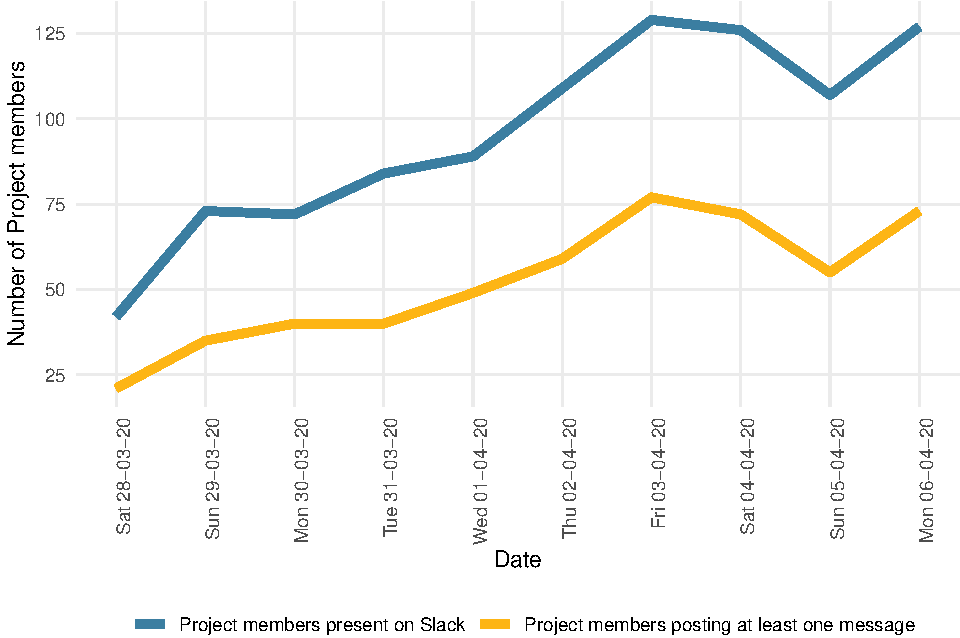
\includegraphics{corona_wp_files/figure-latex/members-1.pdf}
\caption{\label{fig:members}Plot of the number of Project Members present and active on Slack over time}
\end{figure}

\hypertarget{post-data-collection-validation-checks}{%
\subsection{Post-Data Collection Validation Checks}\label{post-data-collection-validation-checks}}

Lastly, we take the following steps in order to validate the quality of the resulting data collected:

\begin{enumerate}
\def\labelenumi{\arabic{enumi}.}
\item
  First, we sample 10\% of the dataset, using the source of the data (e.g.~newspaper article, government press release) as our unit of randomization, to validate. We use the source as our unit of randomization because one source may detail many different policy types.
\item
  Then we then provide these sources to RAs and ask them to code for the government policy based on these sources in a separate, but virtually identical survey instrument. If the source is in a language the RA cannot read, then a new source is drawn.
\item
  We then check for discrepancies between the originally coded data and the second coding of the data in terms of both the number of policies coded and the content of what is coded. If there are no discrepancies, then we consider the data valid. If an RA was found to have made a mistake, then we sample X entries which correspond to the type of mistake made (e.g.~if the RA incorrectly codes an `External Border Restriction' as a `Quarantine', we sample 5 entries where the RA has coded a policy as being about a `Quarantine') and randomly sample X more entries, to ascertain whether the mistake was systematic in nature or not.
\end{enumerate}

Our validation checks reveal that {[}\ldots{}{]}

\hypertarget{dataset}{%
\section{Dataset}\label{dataset}}

Here we present some descriptive statistics to illustrate the type of data that the CoronaNet project is able to provide. Table \ref{tab:desctab} shows the number of records for each policy type, the number of unique countries for each policy type, and also how many countries are targeted in total by each policy type. We would note that these are cumulative totals for these different categories in the data.

\begin{table}[!h]

\caption{\label{tab:desctab}Descriptive Information about the CoronaNet Government Response Dataset}
\centering
\begin{tabular}{>{\raggedright\arraybackslash}p{4cm}>{\raggedleft\arraybackslash}p{2.5cm}>{\raggedleft\arraybackslash}p{2.5cm}>{\raggedleft\arraybackslash}p{2.5cm}>{\raggedleft\arraybackslash}p{2.5cm}}
\toprule
Type & Total Number of Policies & Number of Countries & Number of Targeted Countries & \% With Mandatory Enforcement\\
\midrule
\rowcolor{gray!6}  Closure of Schools & 1050 & 142 & 1 & 87\\
Curfew & 131 & 68 & 13 & 96\\
\rowcolor{gray!6}  Declaration of Emergency & 249 & 92 & 1 & 80\\
External Border Restrictions & 3446 & 172 & 214 & 90\\
\rowcolor{gray!6}  Health Monitoring & 503 & 79 & 201 & 73\\
\addlinespace
Health Resources & 888 & 102 & 105 & 45\\
\rowcolor{gray!6}  Health Testing & 119 & 59 & 48 & 67\\
Internal Border Restrictions & 195 & 83 & 75 & 88\\
\rowcolor{gray!6}  New Task Force or Bureau & 161 & 76 & 1 & 43\\
Other Policy Not Listed Above & 352 & 98 & 1 & 58\\
\addlinespace
\rowcolor{gray!6}  Public Awareness Campaigns & 249 & 97 & 1 & 19\\
Quarantine & 1480 & 133 & 190 & 88\\
\rowcolor{gray!6}  Restriction of Non-Essential Businesses & 867 & 100 & 1 & 89\\
Restriction of Non-Essential Government Services & 119 & 67 & 1 & 78\\
\rowcolor{gray!6}  Restrictions of Mass Gatherings & 421 & 138 & 2 & 86\\
\addlinespace
Social Distancing & 277 & 100 & 2 & 70\\
\bottomrule
\end{tabular}
\end{table}

In addition, we can look at the cumulative indicidence of different types of policies in our data over time, as we show in Figure \ref{fig:overtime}. The figure shows that relatively easy to implement policies like the forming of task forces, public awareness campaigns, and efforts to increase health resources came relatively early. More restrictive policies like curfews, closures of schools and mass gatherings arrived later in the course of the pandemic.

\begin{figure}
\centering
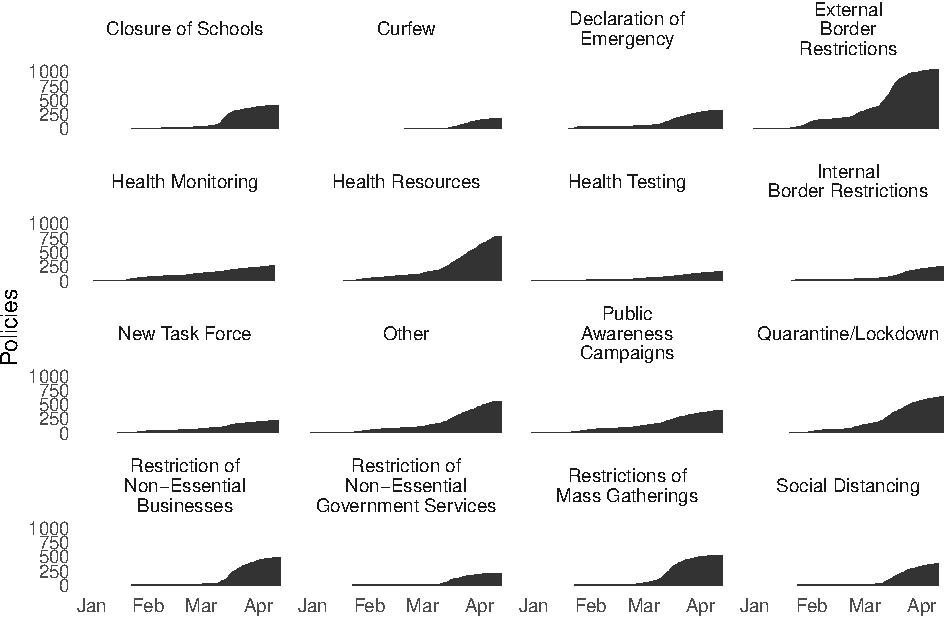
\includegraphics{corona_wp_files/figure-latex/overtime-1.pdf}
\caption{\label{fig:overtime}Cumulative Incidence of Policy Event Types Over Time}
\end{figure}

Of the 4695 events in the dataset, we have identified 4026 unique events. That is, some events in the database are updates or changes to existing policies. We link such events overtime using a unique ID (\texttt{record\_id}). An event counts as an update if it deals with a change in either the:

\begin{enumerate}
\def\labelenumi{\arabic{enumi}.}
\tightlist
\item
  Time duration or\footnote{An example of (1) is if Germany lengthens its quarantine to 28 days from 14 day.}
\item
  Strength of an existing policy in terms of either\footnote{Examples with regards to (2) is if Germany changes the stringency of an existing quarantine such that: (a) people can no longer leave their houses to go to work whereas before they could (b) the quarantine used to be voluntary but now its mandatory (c) the quarantine used to apply to everyone and now it only applies to the elderly.}

  \begin{enumerate}
  \def\labelenumii{\alph{enumii}.}
  \tightlist
  \item
    the nature of the policy
  \item
    compliance rules for the policy
  \item
    who the policy applies towards, if applicable.
  \end{enumerate}
\end{enumerate}

A policy counts as a new entry and not an update if it deals with a change in any other dimension, e.g.~policy type, targeted country.

\hypertarget{government-response-severity-index}{%
\section{Government Response Severity Index}\label{government-response-severity-index}}

In this section we briefly present our new index for tracking the relative intensity of government policies targeting COVID-19 across countries and over time. The model is a version of item-response theory that incorporates over-time trends {[}@kubinec2019ideal{]}, permitting inference on how a latent construct, in this case policy stringency, is responding to changes in the pandemic. To fit the model, the different policy types shown in Table \ref{tab:desctab} were coded dichotomously, with a value of 1 if enforcement of the policy was mandatory, and 0 otherwise. As a result, the model estimates whether mandatory policies for each category exist for each country on each day. The country-level stringency score is allowed to vary over time in a random-walk process with a country-specific variance parameter (i.e., to incorporate heteroskedasticity).

The advantage of employing a statistical model, rather than simply summing across policies, is that the index ends up as a weighted average, where the weights are derived by how likely it is that a certain policy is enforced. In other words, while many countries set up task forces, relatively few imposed curfews at an early stage. As a result, the model adjusts for these distinctions, producing a score that aggregates across the patterns in the data.

Furthermore, because the model is stochastic, it is robust to coding errors. As we discuss in our validation section, while we are continuing to validate the data on a daily basis, the massive speed and scope of data collection means that we cannot identify all issues with the data. However, the measurement model employed only requires us to assume that on average the policy codings are correct, not that they are correct for each instance. Coding error, such as incorrectly selecting a policy type, will propogate through the model as higher uncertainty intervals, but will not affect average posterior estimates. As our data quality improves, and we are able to collect more data over time, the model will produce more variegated estimates with smaller uncertainty intervals.

Figure \ref{fig:plotindex} shows the estimated index scores for the 0 countries in our dataset at present. Of course, a caveat with the index is that not all of the possible measures may be coded in the data already due to difficulty in finding the policies in published sources. However, there is still clear differentation within the index in terms of when policies were imposed, with some countries starting to impose policies much earlier than others. Furthermore, there is a clear break about March 1st when countries began to impose more stringent policies across the world.

\begin{figure}
\centering
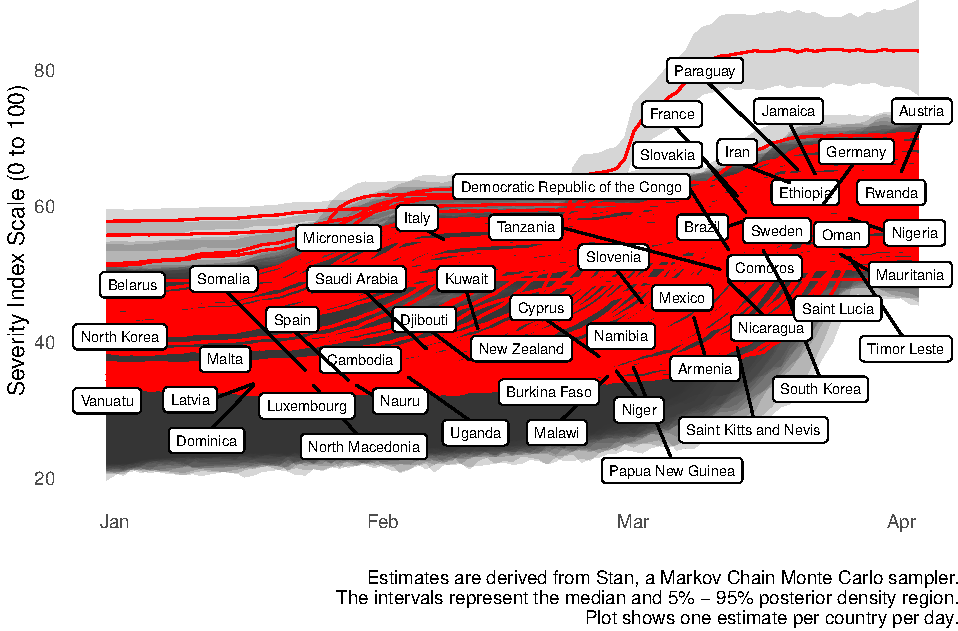
\includegraphics{corona_wp_files/figure-latex/plotindex-1.pdf}
\caption{\label{fig:plotindex}CoronaNet Time-Varying Index of Severity of Measures Opposing COVID-19 Pandemic}
\end{figure}

Table \ref{tab:rankcount} shows the rank of countries for the index at present. San Marino occupies the highest position, likely because of harsh lockdowns imposed as a result of the outbreak in central Italy. Slovenia has had a nationwide lockdown in place for several weeks, while Azerbaijan took early action to close its borders with Iran in February after the outbreak started. It is important to note the uncertainty in the index measures, as the top 10 countries cannot be distinguished from each other in severity except for San Marino. We believe these uncertainty intervals are important to capture the difficulty in using published policies to compare countries. However, we also see substantial value in this index, particularly in its ability to show change over time.

\begin{longtable}{>{\raggedright\arraybackslash}p{4cm}>{\raggedleft\arraybackslash}p{2.5cm}>{\raggedleft\arraybackslash}p{2.5cm}>{\raggedleft\arraybackslash}p{2.5cm}>{\raggedleft\arraybackslash}p{2.5cm}}
\caption{\label{tab:rankcount}Rank of Countries by Severity Index as of April 3rd, 2020}\\
\toprule
Country & Rank & 5\% Low Score & Median Score & 95\% High Score\\
\midrule
\rowcolor{gray!6}  San Marino & 1 & 76.3 & 82.8 & 90.4\\
Slovenia & 2 & 67.5 & 70.6 & 74.8\\
\rowcolor{gray!6}  Azerbaijan & 3 & 67.3 & 70.5 & 73.7\\
Ireland & 4 & 66.9 & 70.3 & 73.8\\
\rowcolor{gray!6}  Poland & 5 & 66.5 & 69.5 & 72.5\\
\addlinespace
Cuba & 6 & 66.3 & 69.2 & 72.4\\
\rowcolor{gray!6}  Argentina & 7 & 65.4 & 68.9 & 72.6\\
Mexico & 8 & 65.2 & 68.8 & 72.4\\
\rowcolor{gray!6}  Denmark & 9 & 65.5 & 68.7 & 71.9\\
Romania & 10 & 65.7 & 68.6 & 71.9\\
\addlinespace
\rowcolor{gray!6}  Ecuador & 11 & 65.1 & 68.5 & 72.4\\
Netherlands & 12 & 64.4 & 67.6 & 71.1\\
\rowcolor{gray!6}  Croatia & 13 & 65.2 & 67.6 & 70.5\\
Israel & 14 & 64.8 & 67.4 & 70.3\\
\rowcolor{gray!6}  El Salvador & 15 & 64.6 & 67.0 & 70.3\\
\addlinespace
Cyprus & 16 & 63.9 & 67.0 & 70.2\\
\rowcolor{gray!6}  Myanmar & 17 & 63.9 & 66.5 & 69.5\\
Saint Kitts and Nevis & 18 & 62.9 & 66.1 & 69.4\\
\rowcolor{gray!6}  Colombia & 19 & 63.2 & 66.0 & 68.8\\
Hong Kong & 20 & 63.5 & 65.7 & 68.0\\
\addlinespace
\rowcolor{gray!6}  Paraguay & 21 & 62.5 & 65.5 & 68.2\\
Jamaica & 22 & 62.7 & 65.3 & 67.8\\
\rowcolor{gray!6}  Madagascar & 23 & 62.1 & 65.1 & 68.4\\
Tanzania & 24 & 62.1 & 65.0 & 67.8\\
\rowcolor{gray!6}  Burkina Faso & 25 & 61.9 & 64.9 & 67.7\\
\addlinespace
Austria & 26 & 62.1 & 64.9 & 67.8\\
\rowcolor{gray!6}  Latvia & 27 & 62.0 & 64.8 & 67.8\\
Albania & 28 & 61.7 & 64.7 & 67.5\\
\rowcolor{gray!6}  Iran & 29 & 62.3 & 64.7 & 67.4\\
Czechia & 30 & 62.1 & 64.4 & 67.2\\
\addlinespace
\rowcolor{gray!6}  Kuwait & 31 & 61.6 & 64.4 & 67.1\\
Egypt & 32 & 61.8 & 64.3 & 66.9\\
\rowcolor{gray!6}  Estonia & 33 & 61.2 & 64.2 & 67.0\\
United Arab Emirates & 34 & 61.5 & 64.1 & 66.9\\
\rowcolor{gray!6}  Zambia & 35 & 61.2 & 64.0 & 67.2\\
\addlinespace
Italy & 36 & 61.8 & 64.0 & 66.3\\
\rowcolor{gray!6}  Niger & 37 & 61.0 & 63.9 & 66.7\\
Djibouti & 38 & 61.0 & 63.8 & 66.5\\
\rowcolor{gray!6}  Somalia & 39 & 61.0 & 63.6 & 66.3\\
Luxembourg & 40 & 61.2 & 63.6 & 66.4\\
\addlinespace
\rowcolor{gray!6}  Bahamas & 41 & 61.1 & 63.5 & 66.2\\
Mongolia & 42 & 61.2 & 63.5 & 66.2\\
\rowcolor{gray!6}  Ukraine & 43 & 61.1 & 63.5 & 66.2\\
Sudan & 44 & 60.7 & 63.4 & 66.6\\
\rowcolor{gray!6}  Ghana & 45 & 60.9 & 63.4 & 66.0\\
\addlinespace
Iceland & 46 & 60.6 & 63.1 & 66.1\\
\rowcolor{gray!6}  Democratic Republic of the Congo & 47 & 60.5 & 63.1 & 65.9\\
Uganda & 48 & 60.5 & 63.1 & 65.7\\
\rowcolor{gray!6}  North Macedonia & 49 & 60.5 & 63.0 & 65.9\\
Honduras & 50 & 60.3 & 62.9 & 65.5\\
\addlinespace
\rowcolor{gray!6}  Canada & 51 & 61.0 & 62.9 & 65.1\\
Monaco & 52 & 60.5 & 62.9 & 65.6\\
\rowcolor{gray!6}  Iraq & 53 & 60.6 & 62.9 & 65.0\\
France & 54 & 60.4 & 62.9 & 65.5\\
\rowcolor{gray!6}  Sweden & 55 & 60.2 & 62.8 & 65.5\\
\addlinespace
Chile & 56 & 59.8 & 62.7 & 65.4\\
\rowcolor{gray!6}  Bhutan & 57 & 59.9 & 62.7 & 65.3\\
Taiwan & 58 & 60.4 & 62.6 & 65.0\\
\rowcolor{gray!6}  Liechtenstein & 59 & 59.9 & 62.6 & 65.2\\
Belgium & 60 & 59.9 & 62.6 & 65.3\\
\addlinespace
\rowcolor{gray!6}  Pakistan & 61 & 60.2 & 62.4 & 64.6\\
Belarus & 62 & 60.1 & 62.4 & 64.7\\
\rowcolor{gray!6}  Sierra Leone & 63 & 59.9 & 62.4 & 65.1\\
Vietnam & 64 & 60.3 & 62.4 & 64.5\\
\rowcolor{gray!6}  Algeria & 65 & 60.0 & 62.4 & 65.1\\
\addlinespace
Trinidad and Tobago & 66 & 60.2 & 62.3 & 64.4\\
\rowcolor{gray!6}  Papua New Guinea & 67 & 59.4 & 62.3 & 65.2\\
Malawi & 68 & 59.5 & 62.2 & 65.0\\
\rowcolor{gray!6}  Russia & 69 & 60.2 & 61.9 & 63.6\\
Panama & 70 & 59.3 & 61.8 & 64.4\\
\addlinespace
\rowcolor{gray!6}  Mali & 71 & 59.2 & 61.8 & 64.4\\
Comoros & 72 & 59.0 & 61.6 & 64.2\\
\rowcolor{gray!6}  Tonga & 73 & 58.8 & 61.3 & 63.4\\
Switzerland & 74 & 58.5 & 61.2 & 63.6\\
\rowcolor{gray!6}  Germany & 75 & 59.0 & 61.2 & 63.4\\
\addlinespace
Indonesia & 76 & 59.1 & 61.2 & 63.5\\
\rowcolor{gray!6}  Saudi Arabia & 77 & 58.9 & 61.2 & 63.8\\
Namibia & 78 & 58.4 & 61.2 & 63.7\\
\rowcolor{gray!6}  Guyana & 79 & 58.5 & 61.2 & 63.7\\
Lithuania & 80 & 59.0 & 61.0 & 63.4\\
\addlinespace
\rowcolor{gray!6}  Central African Republic & 81 & 57.9 & 60.8 & 63.9\\
Rwanda & 82 & 58.4 & 60.8 & 63.2\\
\rowcolor{gray!6}  Ethiopia & 83 & 58.3 & 60.8 & 63.1\\
Fiji & 84 & 58.2 & 60.6 & 63.1\\
\rowcolor{gray!6}  Mozambique & 85 & 58.2 & 60.6 & 63.1\\
\addlinespace
Finland & 86 & 57.9 & 60.5 & 63.1\\
\rowcolor{gray!6}  Malta & 87 & 58.3 & 60.4 & 62.8\\
Singapore & 88 & 58.9 & 60.3 & 61.8\\
\rowcolor{gray!6}  Brazil & 89 & 58.1 & 60.3 & 62.3\\
Solomon Islands & 90 & 57.5 & 60.1 & 62.5\\
\addlinespace
\rowcolor{gray!6}  Angola & 91 & 57.9 & 60.1 & 62.3\\
Jordan & 92 & 57.1 & 59.9 & 62.4\\
\rowcolor{gray!6}  Greece & 93 & 57.7 & 59.8 & 62.2\\
Kenya & 94 & 57.0 & 59.5 & 61.8\\
\rowcolor{gray!6}  Morocco & 95 & 57.3 & 59.5 & 61.3\\
\addlinespace
Bulgaria & 96 & 56.7 & 59.3 & 61.8\\
\rowcolor{gray!6}  Slovakia & 97 & 56.3 & 59.2 & 61.6\\
Afghanistan & 98 & 56.5 & 59.1 & 61.7\\
\rowcolor{gray!6}  China & 99 & 57.4 & 59.1 & 61.3\\
Timor Leste & 100 & 55.7 & 58.9 & 62.0\\
\addlinespace
\rowcolor{gray!6}  Saint Vincent and the Grenadines & 101 & 56.1 & 58.7 & 61.1\\
New Zealand & 102 & 54.8 & 58.5 & 61.3\\
\rowcolor{gray!6}  India & 103 & 55.7 & 58.5 & 60.6\\
Burundi & 104 & 55.4 & 58.4 & 61.0\\
\rowcolor{gray!6}  Nigeria & 105 & 55.2 & 58.3 & 60.8\\
\addlinespace
Dominica & 106 & 54.9 & 58.2 & 61.1\\
\rowcolor{gray!6}  Moldova & 107 & 54.9 & 58.2 & 60.8\\
Nauru & 108 & 54.9 & 58.0 & 60.8\\
\rowcolor{gray!6}  Guatemala & 109 & 55.4 & 57.9 & 60.0\\
Australia & 110 & 54.6 & 57.4 & 59.5\\
\addlinespace
\rowcolor{gray!6}  Uzbekistan & 111 & 54.4 & 57.3 & 59.6\\
Ivory Coast & 112 & 53.6 & 57.2 & 59.9\\
\rowcolor{gray!6}  Kazakhstan & 113 & 54.7 & 57.1 & 60.0\\
Botswana & 114 & 53.3 & 57.1 & 59.8\\
\rowcolor{gray!6}  Bangladesh & 115 & 53.9 & 56.9 & 60.0\\
\addlinespace
Micronesia & 116 & 53.6 & 56.7 & 59.3\\
\rowcolor{gray!6}  Tuvalu & 117 & 53.7 & 56.5 & 59.0\\
Guinea & 118 & 52.1 & 56.1 & 59.5\\
\rowcolor{gray!6}  Peru & 119 & 51.9 & 55.2 & 58.7\\
Hungary & 120 & 52.0 & 55.2 & 57.7\\
\addlinespace
\rowcolor{gray!6}  Armenia & 121 & 51.5 & 55.1 & 58.9\\
Oman & 122 & 51.1 & 55.1 & 58.3\\
\rowcolor{gray!6}  Kiribati & 123 & 51.6 & 55.0 & 57.7\\
European Union & 124 & 50.7 & 55.0 & 58.3\\
\rowcolor{gray!6}  Japan & 125 & 52.1 & 55.0 & 57.7\\
\addlinespace
Cambodia & 126 & 51.1 & 55.0 & 58.3\\
\rowcolor{gray!6}  United States & 127 & 51.7 & 55.0 & 58.6\\
Vanuatu & 128 & 50.9 & 54.9 & 58.2\\
\rowcolor{gray!6}  Mauritania & 129 & 50.7 & 54.9 & 58.4\\
Mauritius & 130 & 50.7 & 54.7 & 58.4\\
\addlinespace
\rowcolor{gray!6}  Spain & 131 & 50.4 & 54.4 & 58.2\\
Saint Lucia & 132 & 51.1 & 54.3 & 57.4\\
\rowcolor{gray!6}  Turkey & 133 & 49.8 & 53.8 & 57.8\\
Lebanon & 134 & 48.7 & 53.6 & 57.7\\
\rowcolor{gray!6}  South Africa & 135 & 48.2 & 53.2 & 57.3\\
\addlinespace
Nepal & 136 & 48.2 & 52.8 & 56.6\\
\rowcolor{gray!6}  Costa Rica & 137 & 48.8 & 52.3 & 55.5\\
Nicaragua & 138 & 46.8 & 51.8 & 55.5\\
\rowcolor{gray!6}  Grenada & 139 & 46.0 & 51.4 & 55.5\\
North Korea & 140 & 47.9 & 51.1 & 54.6\\
\addlinespace
\rowcolor{gray!6}  Maldives & 141 & 45.5 & 50.7 & 55.2\\
South Korea & 142 & 46.5 & 49.2 & 51.5\\
\bottomrule
\end{longtable}

\hypertarget{conclusion}{%
\section{Conclusion}\label{conclusion}}

As policymakers, researchers and the broader public debate and compare how to succeed against the novel threats posed by COVID-19, they need real-time, traceable data on government policies in order to understand which of these policies are effective, and under what conditions. This requires specific knowledge of the variation in policies and their implementation. The goal of the dataset and severity index presented hereis to provide this information.

We have tried to match our data collection efforts to keep up with the exponential speed with which the corona-virus has already upended global public health and the international economy while also mainting high levels of quality. However, we will inevitably be refining, revising and updating our data to reflect new knowledge and trends as the pandemic unfolds. The data that we present in this first version of the dataset represents only our initial efforts and we anticipate making ongoing improvements to the dataset over time.

In future work, the CoronaNet team will also provide their own analyses of what drives these responses, under what conditions they can stymy the epidemic, etc., so as to contribute to the social science research community and provide urgently needed knowledge for policymakers and the wider global community.

\hypertarget{appendix}{%
\subsection*{Appendix}\label{appendix}}
\addcontentsline{toc}{subsection}{Appendix}

\hypertarget{codebook}{%
\subsection*{Codebook}\label{codebook}}
\addcontentsline{toc}{subsection}{Codebook}


\end{document}
